\chapter{Introduction}
\label{chapter:introduction}

%%% SECTION



\section{Motivation}

%%%%%%%%%%%%%%%%%%%
%%% Motivation %%%
%%%%%%%%%%%%%%%%%%%
This journey towards the elaboration of this exciting work on dermoscopic classification of skin disease is a path that combines science, technology and medical care uniquely. 

Artificial Intelligence (AI) is bringing about a fourth industrial revolution that is already affecting our society. In concrete, its incorporation into medicine has a very significant impact on different medical areas (\cite{luciaclemares_que_2023} y \cite{apd_aplicaciones_IA_Medicina}) such as:

\begin{itemize}
    \item \textbf{A more accurate and organised diagnosis}: The use of advanced search techniques on large medical data sets allows for more accurate and reliable diagnostic. 
    \item \textbf{Faster and more efficient drug development}: Accelerating the research and development of new drugs.
    \item \textbf{Personalised care}: AI can customise treatment plans for each patient's individual needs optimising, at the same time, effectiveness and minimising side effects.
    \item \textbf{Images diagnostic more accurate and faster}. The worldwide name of AI will be recognised henceforth in this work as Deep networks. A part of these networks is specialised image recognition. They have a pattern detection capability that is by far superior to any human being. They can also make a diagnosis with very little delay. For the aforementioned reasons, it will be an essential tool for improving patient care and treatment. 
\end{itemize}

This last point is the core of the scope of this project. Personally, this project is much more than a task for ending a long master's journey. This job represents a challenge because working with large image files requires pre-processed data. In addition to this, the model to be developed is a classification one that should distinguish among nine different patterns.

It also represents an opportunity to imagine that my work could be helpful, one day, in the early detection of multiple skin diseases, and thus improve medical care and services.



\section{Goals}

%%%%%%%%%%%%%%%%%%%
%%% Goals %%%
%%%%%%%%%%%%%%%%%%%

This project's main objective is the classification of dermoscopic images in order to identify nine types of skin lesions. To achieve this a Convolutional Neural Network (CNN) will be created. This challenge can be separated into two goals.

\begin{itemize}
    \item On the one hand, to analyse the current \textbf{state of the art} in automatic medical detection by imaging.
    \item Secondly, to \textbf{classify these lesions into one of nine classes} to be studied.
\end{itemize}

In parallel, the dataset contains a metadata file. This information can help to segment the source information according to the types of dermoscopic techniques used. Therefore, this provides us with a \textbf{secondary objective} by allowing us to make a reliability ranking according to the technique used. 


\section{Methodology}

%%%%%%%%%%%%%%%%%%%
%%% Methodology %%%
%%%%%%%%%%%%%%%%%%%

For the implementation of this project, we will use the Cross Industry Standard Process for Data Mining or \textbf{CRISP-DM} methodology. This methodology consists of six phases that are cyclically carried out and it allows feedback to previous phases in order to complement the deficiencies of other phases. The following diagram (figure 1.1) shows the six-phase cyclical circuit to be used in this methodology.

\begin{figure}[ht]
    \begin{center}
        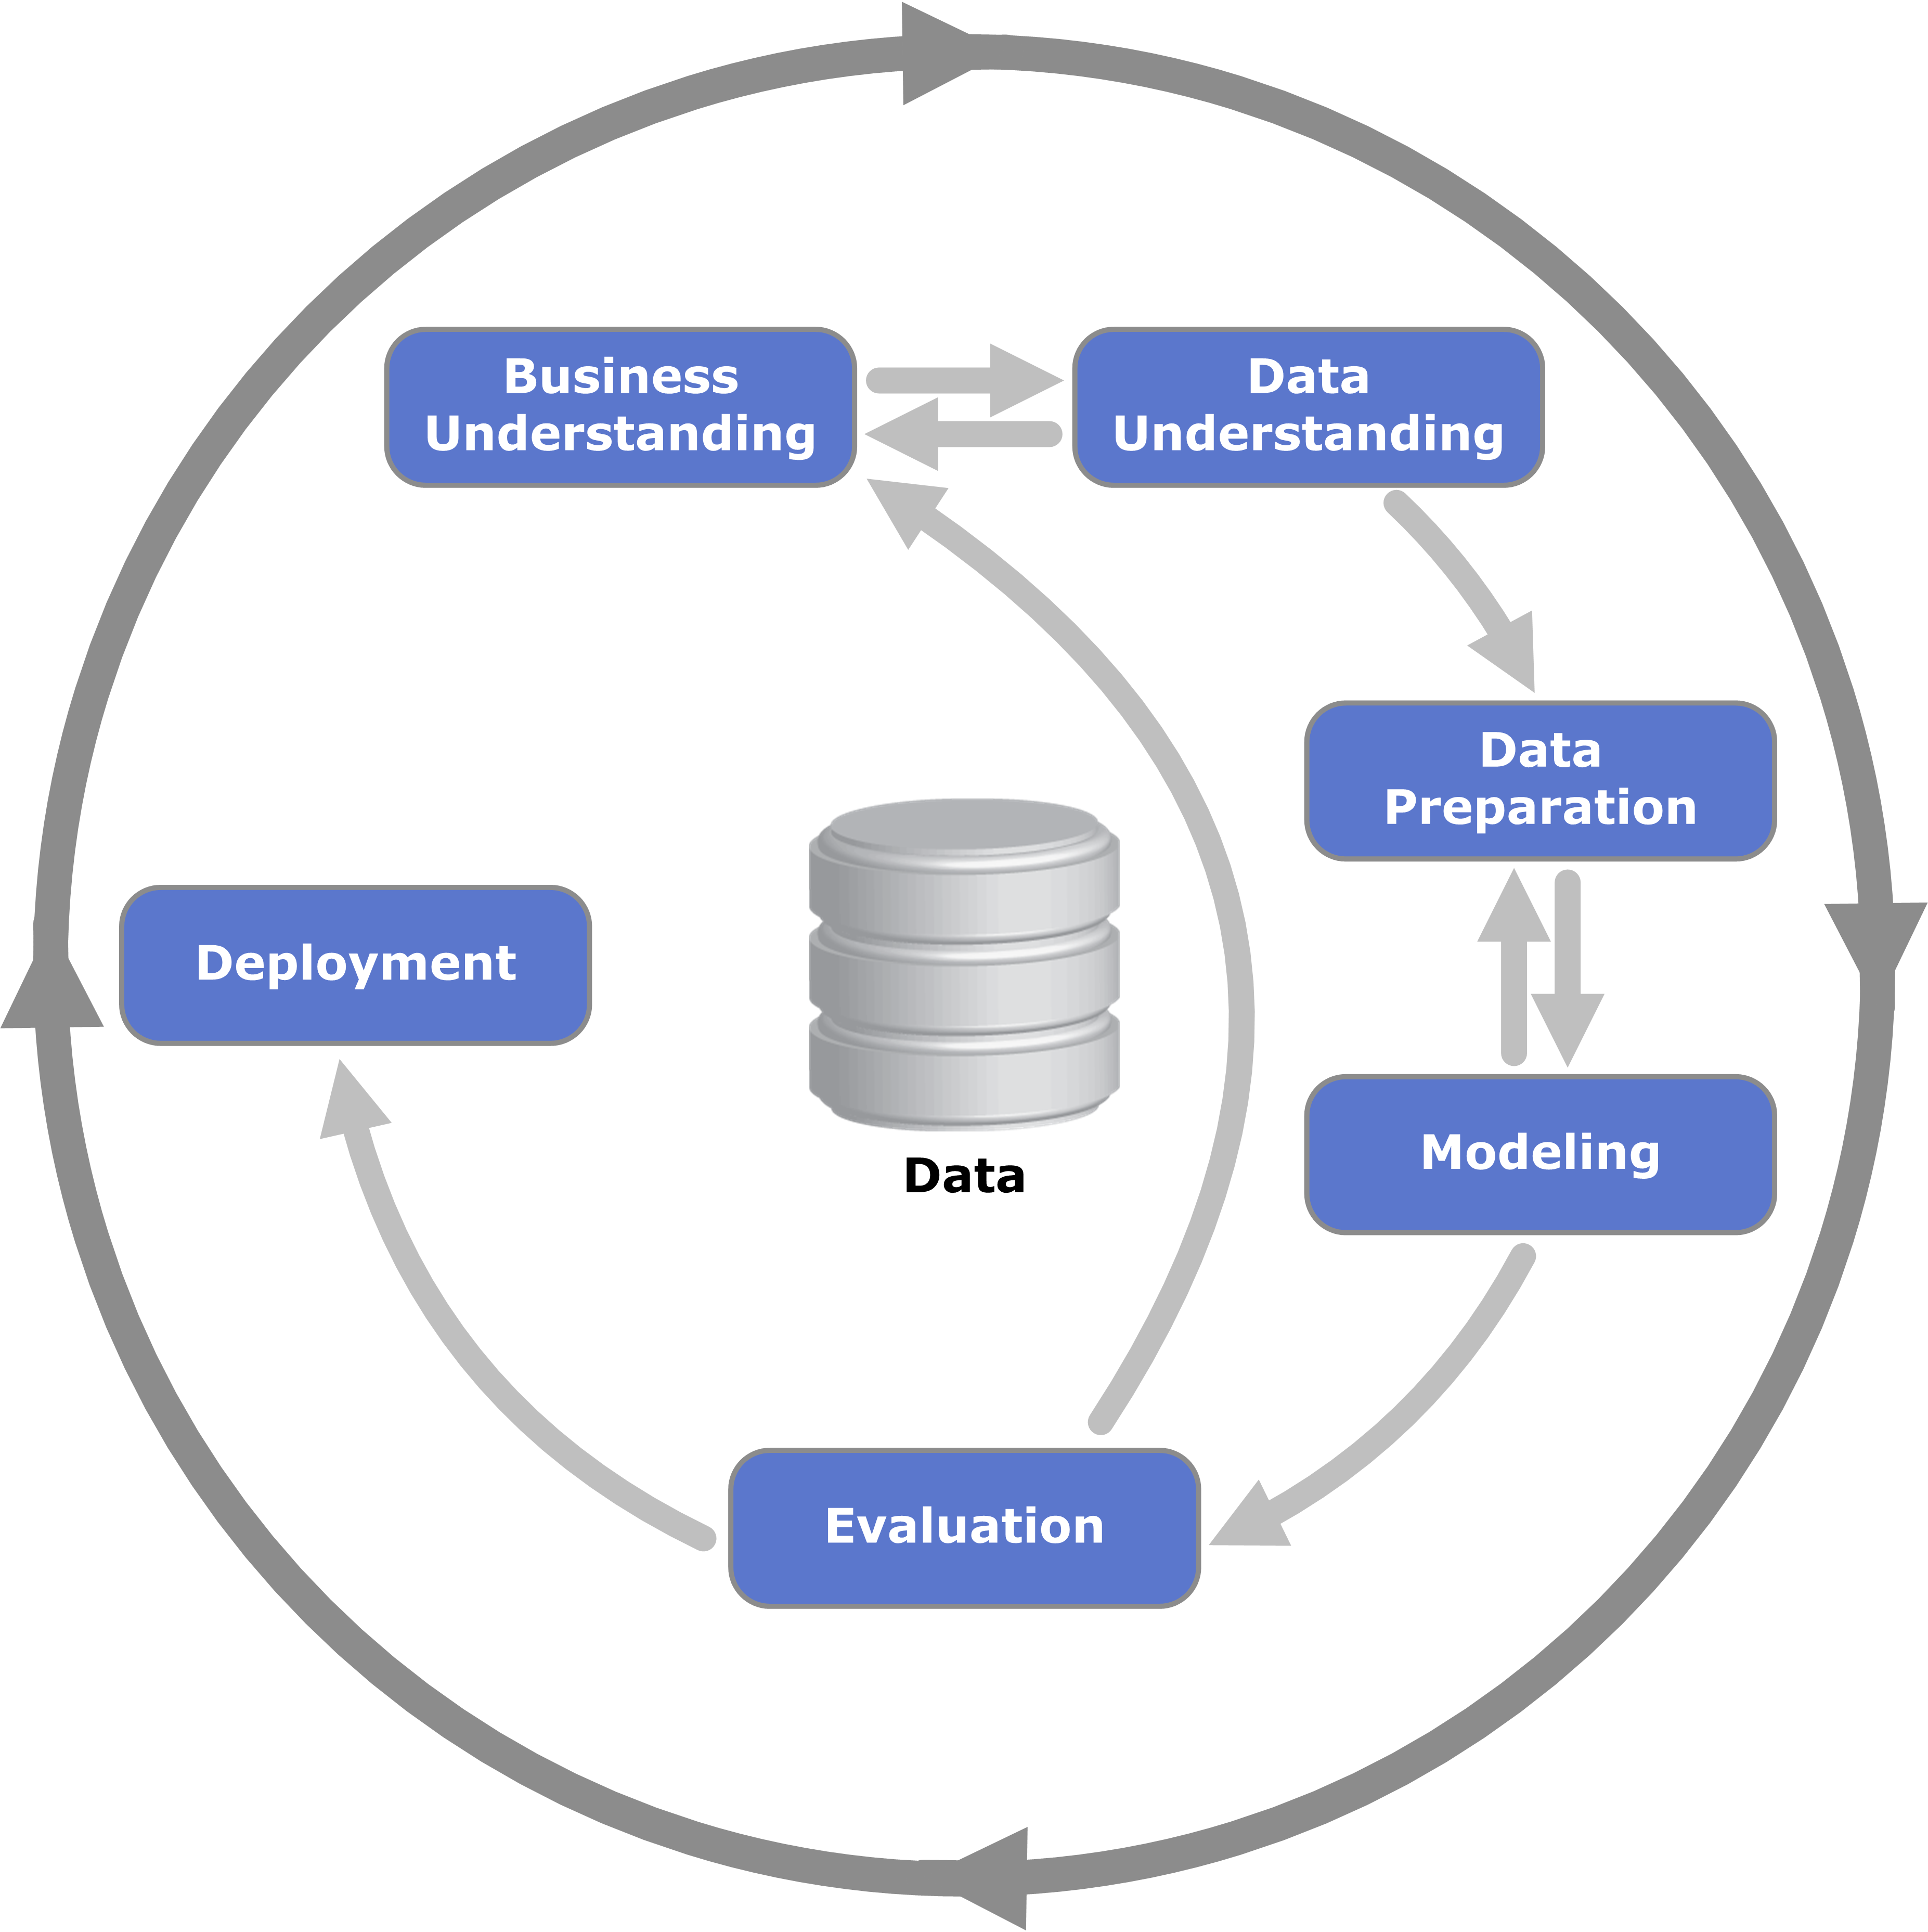
\includegraphics[scale=0.60]{images/CRISP-DM_Process_Diagram.png}
        \caption{Process diagram showing the phases of the CRISP-DM methodology}
    \label{fig:CRISP-DM}    
    \end{center}
\end{figure}


The methodology phases and the adaptation to the project are described below:

\begin{enumerate}
    \item \textbf{Business understanding}
    
    The first phase of the \textbf{CRISP-DM} model starts understanding the project's main objectives. These are mentioned in the \textbf{ Goals section} above. At this stage of the project, licensing costs are reviewed. Concerning licensing cost in this project there is \textbf{no associated licensing cost}, because the data is left under an open licence (see \textbf{Licensing section}). Furthermore, the project plan is also created during this phase (see \textbf{project plan section}).

    \item \textbf{Data understanding}
    
    Typically, this phase seeks to become familiar with the understanding of the data, identifying quality problems and discover hidden information or interesting subsets of the data to be processed. This allows to have point of view. A key aspect will be to verify the quality, in order to define all required strategies to address them. At the end of this phase, we will already have a conceptual data model.

    As the images to be used as a data source are produced in a medical environment, they are expected to be of high quality. However, this will be validated in the early stages of the project.

        
    \item \textbf{Data Preparation}

    In this section, applying the \textbf{CRISP-DM} method, a selection and integration of the main data together with their required attributes will be carried out. Moreover, data will be cleaned and formatted if required, looking for the main fields or characteristics of the data.

    Our project has the challenge of working with \textbf{large data input} (around 21 GB). Therefore, one of the first tasks will be \textbf{resizing} the data to reduce the size and work with a more manageable dataset. On the contrary, we will look at using some \textbf{data augmentation} techniques to help us avoid overfitting. 
    
    \item \textbf{Modelling}

    In this phase, the modelling techniques required to achieve an optimal data model will be applied. As it is  shown in the phase diagram, it is a phase that usually builds on the data preparation phase, either to solve problems or to enrich the data. Additionally to model building, some model evaluation techniques will be required. As a result, a test plan document will be done.

    
    \item \textbf{Evaluation}

    Once the objectives set requiered, during the initial phases have been obtained, an evaluation must be carried out to ensure that them were reached. This is done using the test plan designed in the previous phase. If necessary, the process will be reviewed and, depending on the results, the next steps will be planned. A benchmark well be carried out amont various models created, and the outstanding model is selected. 

    
    \item \textbf{Deployment}

    At the time, the model has passed all the tests and has been approved, it is required to define a plan for its deployment. Thus, creating a final model is not the end of the project, but rather a milestone within it. A model put into production environment it is necesary to monitor and maintain constantly. Along with the previous, it is advisable to publish results that help to understand whether the objectives initially requested in phase 1 have been achieved. It is quite common that after the project has been put into production, new expectations are generated that make the model (project) generated be reconsidered. This is why \textbf{CRISP-DM} describes the life cycle for the data mining project in a circular framework, where the output feeds back into a new cycle that seeks the continuous improvement of the business.

    Our project is part of a work that will develop a minimum viable product. Finally, the outstanding model will be run on the dataset test to obtain the final metrics.

After the project is structured by phases where no changes are expected in the definition of each one of them, and where the beginnings and ends of each phase are very well defined, a \textbf{waterfall model} is a better approach than other \textbf{agile strategies} for the project follow-up.

    
\end{enumerate}


\section{Planning}

%%%%%%%%%%%%%%%%%%%
%%% Planning %%%
%%%%%%%%%%%%%%%%%%%
The project has been structured in \textbf{five phases} or modules, which in turn are broken down into smaller tasks. This section describes the project's planning and its main milestones. 
\begin{itemize}
    \item \textbf{Module 1 - Project definition} 
    
    This module starts defining the project's plan: the relevant objectives of the project, the initial planning that will form the basis of the project, and the personal motivation to carry out the project on the chosen topic. During this phase, the form "Ethical and personal data protection protocol" will be filled out and presented.
    \item \textbf{Module 2 - State of Art}
    
    During this module time, we will carry out a research phase in which we will search for previous or current scientific work related to this project the main topic. 
    \item \textbf{Module 3 - Design \& implementation}
    
    The objectives of this activity are to implement the tasks necessary for the project's design and development according to the chosen scientific methodology. During this period, the progress made on it will be documented in order to complement the project document. 
    \item \textbf{Module 4 - Document redaction}
    
    This action's purpose is to prepare all the materials required for the presentation and final TFM (Master's Thesis) assessment. These materials include:
    
    \begin{enumerate}
        \item The Master's Thesis document
        \item An audiovisual presentation
    \end{enumerate}

    \item \textbf{Module 5 - Project defence}
    
    Finally, the last step of the Master's Thesis is to defend it before a board of examiners.
\end{itemize}

The following table shows each of the phases, namely: the start and end dates, as well as the estimated effort.


\begin{table}[H]
    \resizebox{\textwidth}{!}{%
    \begin{tabular}{@{}clcccc@{}}
        \toprule
        \textbf{Module}            & \textbf{Description}     & \textbf{Start Date}     & \textbf{End Date}     & \textbf{days} 
   & \textbf{Effort (h)} \\ \midrule
        \textbf{} 1 & Project definition & 09/27/23 & 10/10/23 & 13 & 26 \\
        \textbf{} 2 & State of Art & 10/11/23 & 10/24/23 & 13 & 26 \\
        \textbf{} 3 & Design \& Implementation & 10/25/23 & 12/19/23 & 55  & 110 \\
        \textbf{} 4 & Document redaction & 12/20/23 & 01/16/24 & 27  & 54 \\
        \textbf{} 5 & Project defence & 01/17/24 & 02/03/24 &  17 & 34 \\
        \bottomrule
    \end{tabular}%
    }
    \caption{Project Timetable.}
    \label{table:Timetable}
\end{table}



The time evolution of the project is shown by the following Gantt graph.

\begin{figure}[H]
    \begin{center}
        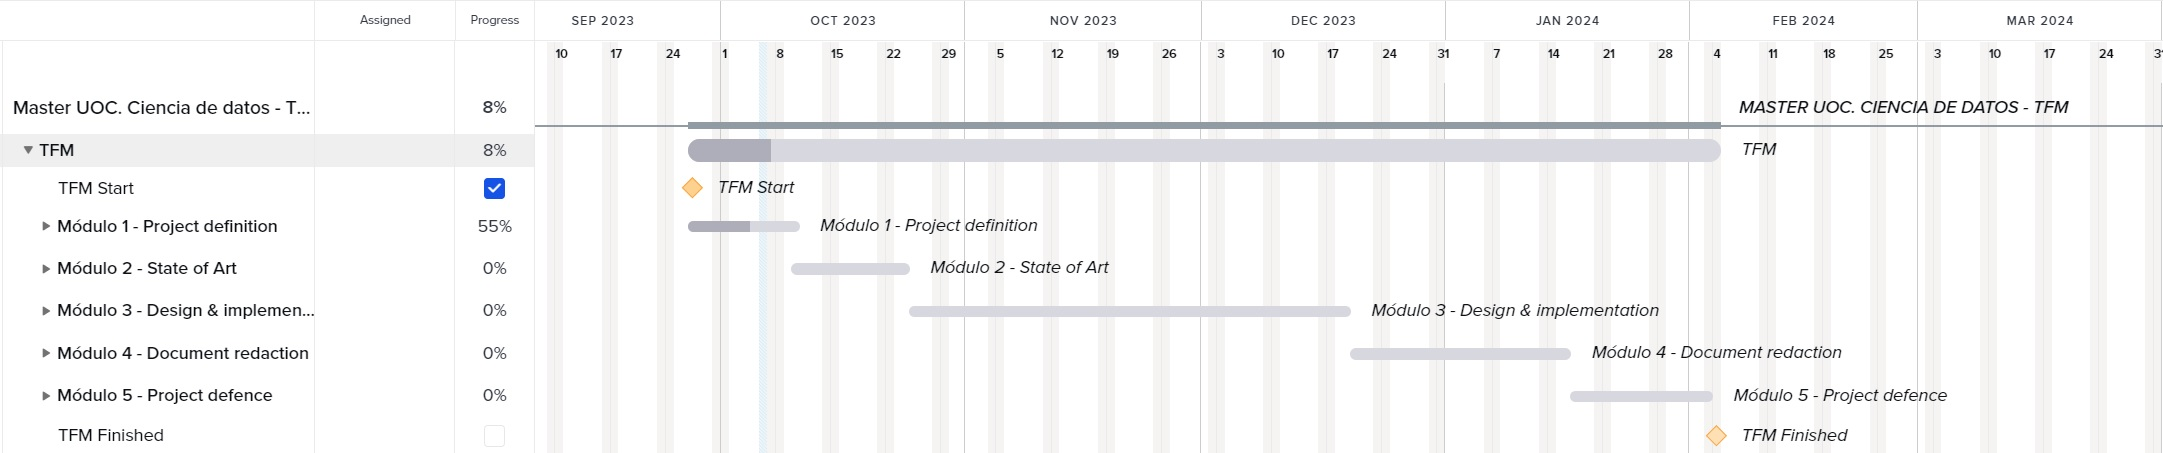
\includegraphics[scale=0.43]{images/TFM_Planing.jpg}
        \caption{Master's final project Gantt's chart}
    \label{fig:Gantt}    
    \end{center}
\end{figure}